\documentclass[12pt,titlepage,french]{article}
\usepackage{babel}
\usepackage{graphicx}
\usepackage[margin=2.5cm]{geometry}
\usepackage{tabularx}
\usepackage[hidelinks]{hyperref}

\usepackage[utf8]{inputenc}
\usepackage[T1]{fontenc}
\pagestyle{plain}

\usepackage{booktabs,makecell,tabu}
\usepackage{float}
\renewcommand\theadfont{\bfseries}

\linespread{1.2}

\begin{document}

\begin{titlepage}
\newcommand{\HRule}{\rule{\linewidth}{0.5mm}}
\center

  
\includegraphics[width=0.45\textwidth]{../ressources/img_logos/logo_polytech.png}\\[1cm]

  
\includegraphics[width=0.45\textwidth]{../ressources/img_logos/logo_taglabs.png}


\HRule \\[0.4cm]
{ \huge \bfseries Description du système \\[0.15cm] }
Classification colorimétrique de nuages de points 3D
\HRule \\[1.5cm]
Ronan Collier,
Mathieu Letrone,
Tri-Thien Truong
\\[1cm]
\today \\ [1cm]
Version 1.0 - Beta
\end{titlepage}

\tableofcontents % table des matières
\newpage
\listoffigures  % table des figures
\newpage
\section{Contexte et problème}

Taglabs est une jeune entreprise créée il y a deux ans par Yan Koch. L’entreprise s’inscrit dans le domaine de la modélisation 3D d’ouvrages. Ils proposent la modélisation et l’exploitation de nuages de points. Toutefois, ils travaillent surtout en interne sur un logiciel « ScanSap », le but de ce logiciel est d’exploiter les nuages de points 3D avec efficacité et simplicité inégalées. \newline

L’entreprise travaille principalement avec les acteurs du BTP et de l’industrie sur des opérations de rénovation et de modernisation des ouvrages. Ces opérations nécessitent de s’appuyer sur des plans qui vont servir aux divers corps d’état pour préparer les travaux.\newline

Par le passé, les plans étaient physiques (plans papier), et sont désormais numériques (plans 2D et maquettes 3D). Ces plans sont malheureusement souvent obsolètes, ce qui est lié aux nombreux petits travaux réalisés au cours de la vie des bâtiments, et qui ne font pas l’objet de mise à jour documentaire. Ceci conduit les entreprises à faire des erreurs dans leurs études techniques, puis des reprises sur site chronophages et coûteuses. \newline

Depuis quelques années, il est possible de faire scanner les bâtiments en 3D et ainsi obtenir un relevé précis sous forme de nuages de points. Le problème rencontré par les entreprises réside dans la difficulté d’exploitation de ces relevés.\newline

\begin{figure}[H]
\center
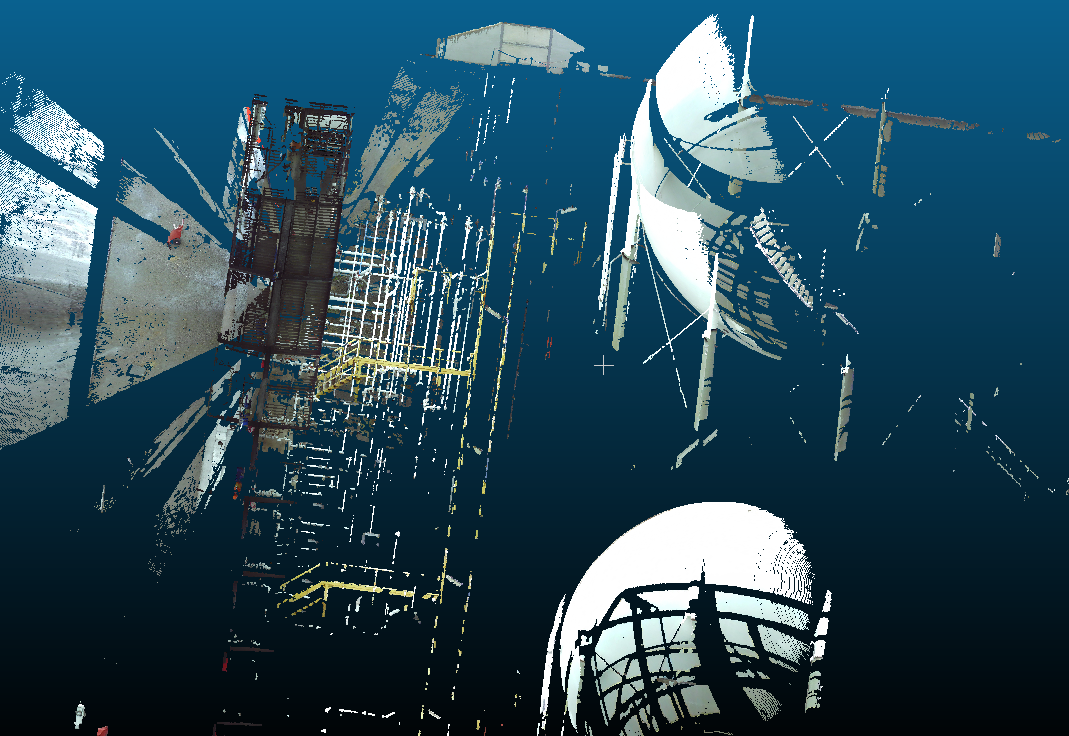
\includegraphics[width=1\textwidth]{./img/exemple_ndp.PNG}
    \caption{\label{} Exemple de nuage de points en 3D}
\end{figure}

Nous pouvons voir ci-dessus, un exemple de nuage de points en 3D, que l'entreprise utilise en tant que données d'entrée. C'est un nuage de points très volumineux, de plus de 22 millions de points. C'est ce type de données que l'entreprise cherche à exploiter au mieux, afin de répondre aux besoins de leurs clients.\newline

TagLabs travaille sur 2 volets :

\begin{itemize}
    \item la conversion du nuage en maquette numérique (CAO / BIM),
    \item l’exploitation du nuage de points tel quel par le biais de fonctionnalités avancées de mesure et de segmentation. \newline
\end{itemize}

C’est ce second volet qui est abordé dans ce projet. \newline

Dans cette optique, l'entreprise souhaite pouvoir intégrer plusieurs fonctionnalités à son système. D'une part, une solution permettant une segmentation basée sur la couleur au sein du ou des nuages de points manipulés. Cette segmentation a pour but de mettre en évidence, isoler les éléments du nuage de point répondant à une plage de couleur demandée. D'autre part, une solution mettant en place une fausse couleur sur un scan (nuage de points) en intensité. Le rôle de la fausse couleur est de mettre en lumière des caractéristiques issu des éléments scannés, et de faciliter la compréhension générale du nuage en y mettant des couleurs. \newline

L'ensemble des fonctionnalités demandées par le client est une demande de recherche algorithmique sur l'implémentation des solutions.

\section{Solution mise en place : vue globale}

Dans cette partie, nous allons présenter l'ensemble des choix que nous avons fait afin de répondre au mieux aux besoins demandés par le client. De plus, nous présenterons la description de la solution conçue pour satisfaire ces besoins.

\subsection{Choix principaux}

Afin de répondre aux besoins, qui sont de pouvoir :
\begin{itemize}
    \item Lire un fichier de données contenant un nuage de point.
    \item Isoler un élément dans le nuage de points, selon sa plage de couleur.
    \item Réaliser de la fausse couleur sur un nuage de points en intensité de gris.
    \item Exporter le nuage de points. \newline
\end{itemize}

Le service proposé doit permettre aux utilisateurs de réaliser ces tâches. Nous avons d'abord défini en tant qu'utilisateurs de la solution, ceux qui utiliseront "ScanSap" qu'il s'agisse de client ou de membre de l'entreprise TagLabs. Ainsi, nous visons des utilisateurs voulant manipuler des nuages de point en 3D. Ces personnes sont équipés de matériels puissants pour faire cela.\newline


N'existant pas d'outil permettant l'ajout direct de fonctionnalités extérieures au sein du logiciel "ScanSap", nous avons décidé avec l'entreprise de réaliser un plugin sur autre logiciel de manipulation de nuages de points. Le logiciel en question est CloudCompare. Il permet la manipulation et le traitement des nuages. De plus, sa licence open source autorise l'ajout de fonctionnalités tant que nous les livrons aussi en open source. \newline

Cette décision fut prise pour répondre non seulement à l'ensemble des besoins, mais aussi car CloudCompare prend déjà en charge deux besoins, la lecture et l'exportation des scans. En faisant ce choix, nous pouvons nous consacrer à la recherche et la réalisation des autres besoins de la segmentation et de la fausse couleur demandés par l'entreprise.

\subsection{Description de la solution}

Comme dit précédemment, la solution proposée pour répondre à la problématique s'articule autour d'un service de type plugin utilisateur. Le plugin est intégré dans les composants tiers de CloudCompare, il comprend (comprendra) les fonctionnalités de segmentation suivant la plage colorimétrique et la génération de fausses couleurs sur un scan en intensité. \newline

Les utilisateurs pourront y accéder en les sélectionnant dans le menu défilant qui liste les différents plugins présents. Les diagrammes de séquence qui suivent, détaillent et illustrent le fonctionnement de l'expérience utilisateur. \newline

La figure 1 montre la démarche que doit suivre l'utilisateur pour avoir accès au plugin.

\begin{figure}[H]
\center
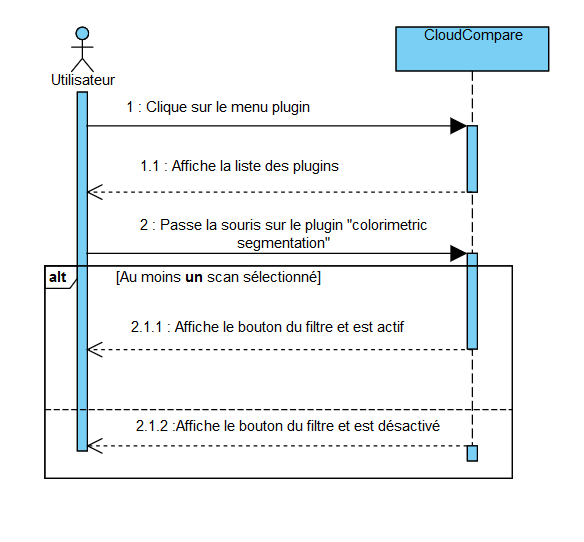
\includegraphics[width=0.65\textwidth]{./img/sequDiagPlugin.PNG}
    \caption{\label{} Diagramme de séquence sur l'accès au plugin}
\end{figure}

La marche à suivre est relativement simple puisque notre plugin s'intègre dans le menu défilant qui répertorie l'ensemble des autres plugins accessibles de CloudCompare. De cette manière, l'utilisateur n'a qu'à le sélectionner et pourra l'utiliser si un ou des nuages ont été choisis pour être traités. \newline

La figure 2, quant à elle, illustre l'utilisation du plugin, plus particulièrement la segmentation colorimétrique.

\begin{figure}[H]
\center
  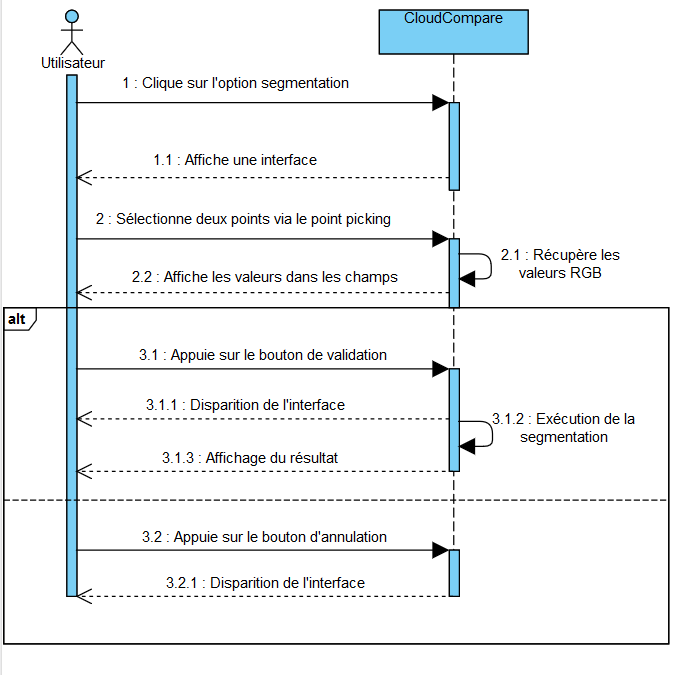
\includegraphics[width=0.65\textwidth]{./img/sequDiagrSegmentation.PNG}
  \caption{\label{} Diagramme de séquence sur l'utilisation de la segmentation}
\end{figure}

L'expérience utilisateur a été revue et s'améliore au fil des retours client à chaque itération. Ainsi, ce diagramme prend en compte les feedbacks de la dernière itération en date, mais sont encore susceptibles d'évoluer jusqu'à la recette. Une fois les étapes de la figure 1 réalisés, une fenêtre apparaît et permet à l'utilisateur de choisir deux points dans le nuage via le point picking de CloudCompare. Ces points serviront pour définir les bornes de la plage colorimétrique des élément qu'il souhaite isoler. Une fois fait, il peut valider son choix via un bouton ou annuler l'opération. \newline

Le tableau ci-dessous présente l'état d'avancement des composants de la solution, en mettant en évidence leur état via un code couleur :
\begin{itemize}
    \item Vert : composant réalisé
    \item Orange : composant en cours de réalisation
    \item Rouge : composant pas encore réalisé
\end{itemize}

\begin{figure}[H]
\center 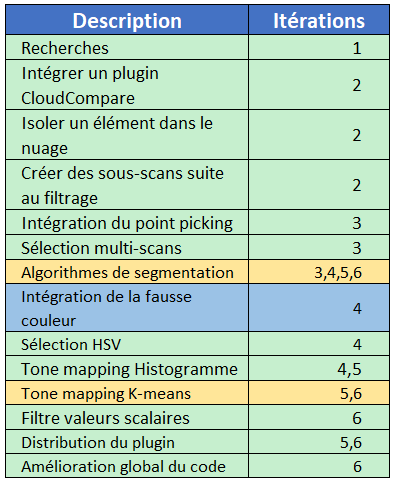
\includegraphics[width=0.5\textwidth]{./img/avancement.png}
  \caption{\label{} Tableau d'avancement global}
\end{figure}

Nous pouvons observer que notre avancement est en bonne voie. Étant à la moitié du projet, nous avons réalisé la moité des tâches. Il faut aussi noter que les composants sont amenés à évoluer, avec le feedback du client à nos fins d'itérations. Par exemple, la tâche du point picking, ou encore le toon mapping sont des composants qui ont été soulevé suite à nos réunions et discussions avec le client et notre tuteur académique.

\section{Description technologique de la solution}

Dans cette partie, nous présenterons les différents composants de l'architecture qui composent notre projet. Nous présenterons également la structure du code, et des différents éléments qui intéragissent sur le projet.

Notre solution étant un plugin pour CloudCompare, la principale difficulté technique est la compréhension de la structure de ce logiciel et de son API. \newline

En effet, CloudCompare possède une structuration complexe pour toute personne qui n'est pas habituée à travailler sur des projets C++ d'une telle envergure.

De plus, la documentation possède de nombreuses lacunes, ne présentant pas toutes les classes et n'étant pas à jour.
Il est donc conseillé de regarder le fonctionnement de l'API en naviguant dans les sources du projet.

\subsection{Structure du code source CloudCompare}

Nous présenterons ici la structure du projet CloudCompare, et de l'implémentation de notre plugin.

\begin{figure}[H]
\center
  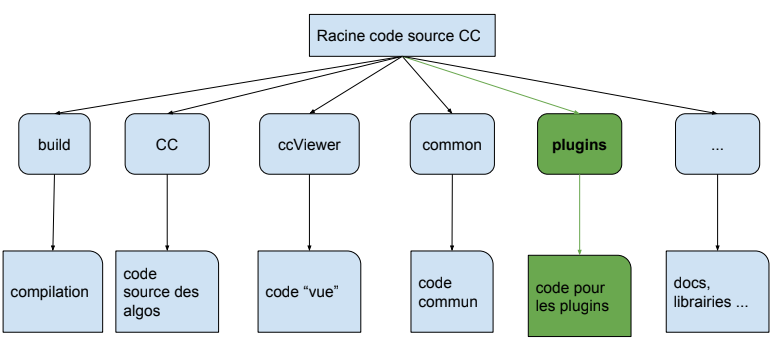
\includegraphics[width=0.9\textwidth]{./img/structure_code.PNG}
  \caption{\label{} Code source du projet CloudCompare}
\end{figure}

Le code source du projet se trouve aux côtés de celui des autres plugins, dans le dossier "plugins" situé à la racine du dossier des sources de CloudCompare (représenté en vert sur la figure ci-dessus). Chaque sous-dossier de ce dossier représente un plugin. \newline

Pour représenter comment les différents composants sont liés ensemble au sein du projet, nous avons utilisé un diagramme de composants. Le plugin se trouve parmi les autres composants tiers à CloudCompare, mais utilise toutes les librairies du cœur de CloudCompare et interface avec le client en passant par le logiciel.

\begin{figure}[H]
\center
  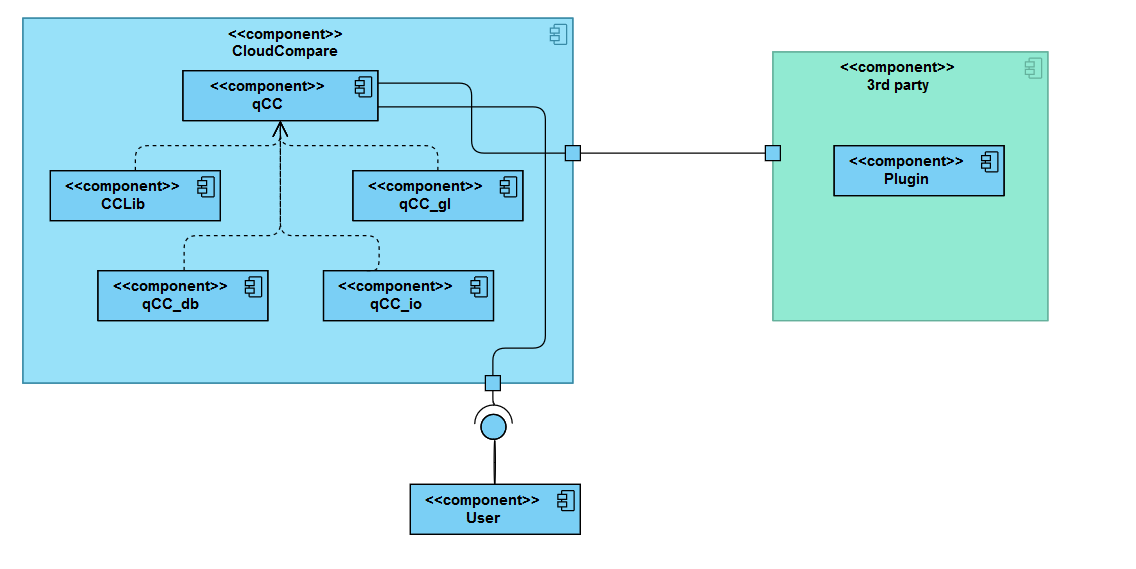
\includegraphics[width=0.9\textwidth]{./img/component_diagr.png}
  \caption{\label{} Diagramme de composants du projet CloudCompare}
\end{figure}

La structure du code source de CloudCompare est organisée pour éviter d'avoir du code éparpillé partout dans le projet original. Nous avons juste à insérer notre code et développer notre propre plugin dans le dossier plugins.

\subsubsection{Projet Cmake}

Le fichier le plus important pour la compilation du projet est le "CMakeLists.txt". En effet, il contient le nom de la classe principale du projet ainsi que tous les fichiers à inclure lors de la compilation.
Si la structure du projet est correcte, et les fichiers correctement configurés, une option sélectionnable apparaît dans CMake.
Il est alors possible de construire le projet pour qu'il soit éditable à l'aide de QtCreator tout autre IDE (tel que Visual Studio, en sélectionnant l'option appropriée).

\subsubsection{Intégration du nouveau plugin dans le projet CloudCompare}

Pour chaque plugin, il faut respecter une certaine structure. Dans le projet CloudCompare, il existe une classe template, qui nous a servi pour la création de notre propre plugin. Il est important de bien le construire, afin de pouvoir interagir avec les éléments du logiciel (graphiquement, et sur les données). \newline

Nous avons représenté la structure globale du plugin, avec ce schéma ci-dessous.

\begin{figure}[H]
\center
  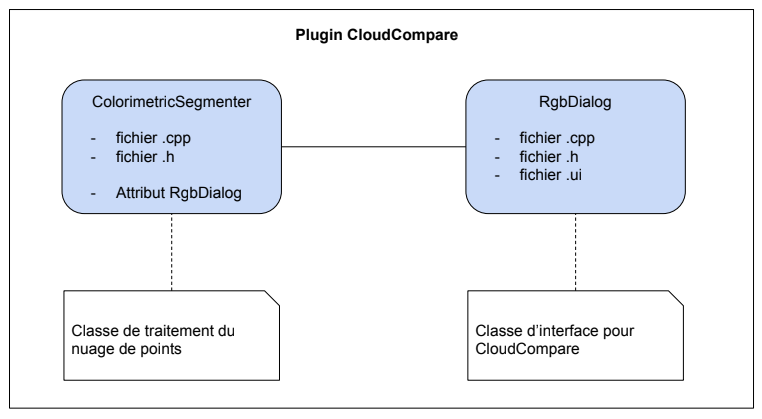
\includegraphics[width=0.9\textwidth]{./img/architecture_plugin.PNG}
  \caption{\label{} Structure de notre plugin}
\end{figure}

Nous pouvons observer que le plugin se compose de deux principales classes. La première, ColorimetricSegmenter, est la classe qui va permettre le traitement des données, et la classe RgbDialog est la classe pour créer l'interface sur CloudCompare.

\subsubsection{Classe de traitement : ColorimetricSegmenter}

Notre classe principale est ainsi nommée "ColorimetricSegmenter". Étant donné que notre projet est en C++, la classe est d'abord représentée sous la forme d'un fichier de type "header", contenant simplement les signatures des méthodes. \newline

Afin de pouvoir interagir avec l'environnement de CloudCompare, il a fallu faire hériter notre classe de la classe "ccStdPluginInterface". Cette dernière est déjà présente dans le projet de base de CloudCompare, et permet de faciliter l'implémentation d'un nouveau plugin. En effet, elle nous permet d'avoir un objet de type "ccMainAppInterface", qui regroupe tous les éléments de la fenêtre, et tous les éléments nécessaires pour interagir sur l'interface. \newline

Cette classe "ColorimetricSegmenter" contient donc tous nos types de filtrage sur le nuage de points. Il contient donc le code permettant d'effecter les actions que l'on veut dans le nuage de points au moment où on valide la fenêtre de paramétrage d'un filtrage. \newline

Afin de faire le lien avec l'interface graphique sur CloudCompare (car dans ce fichier, nous avons uniquement la partie "traitement"), il faut aussi penser à initialiser l'attribut de la classe qui correspond à l'objet de l'interface, dans notre cas, c'est l'attribut de type "RgbDialog".

\subsubsection{Classes d'interface}

L'interface graphique de CloudCompare se base sur la bibliothèque Qt. Cette bibliothèque offre plusieurs moyens afin de créer de nouveaux panneaux d'interface, de les intégrer à l'environnement existant, et de les lier à des actions. \newline

QtCreator permet de concevoir graphiquement un panneau au travers d'une interface intuitive en drag\&drop. Le panneau nouvellement créé peut être enregistré au format XML avec l'extension ".ui". Lors de la génération du projet, des fichiers ".h" et ".cpp" sont automatiquement créés par CloudCompare afin de pouvoir ouvrir la fenêtre et manipuler ses champs. \newline

\begin{figure}[H]
\center
  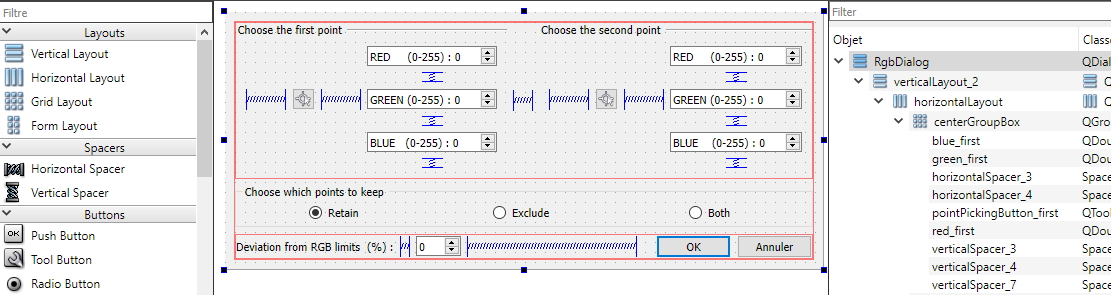
\includegraphics[width=1\textwidth]{./img/qt_creator.PNG}
  \caption{\label{} Exemple QtCreator : RgbDialog}
\end{figure}

Concrètement, nous avons par exemple, un fichier "RgbDialog.ui", créé avec le logiciel Qt Creator. Grâce à ce fichier, en générant le projet, les fichiers "RgbDialog.h" et "RgbDialog.c" se créent. Il est ensuite possible d'ajouter des méthodes dans le fichier "RgbDialog.c" afin d'ajouter des traitements. \newline

Au niveau de l'interface en elle même, il s'agit essentiellement de boutons et de champs de texte. Nous avons essayé de faire des interfaces très simple à comprendre et assez épurée.  \newline

Nous avions rencontré des problèmes pour certains types d'écrans (notamment les écrans 4K), où certains composants avaient du mal à s'afficher. C'est pour cela que grâce aux Spacers (représentés en bleu sur l'image ci-dessus), les composants s'adapent en fonction de la taille de la fenêtre. Chaque utilisateur pourra donc redimensionner la fenêtre selon ses goûts.

\subsubsection{Gestion des actions sur l'interface : Qt}

Les actions utilisateurs sont gérées grâce à Qt au travers de la mécanique des signaux et des slots. Chaque événement, tel que l'ajout d'un nuage de points, est représenté par un slot et un signal. \newline

Notre plugin peut ainsi savoir si l'utilisateur a sélectionné un nuage de points ou non, ou encore s'il clique sur un point. Il est également tout à fait possible de créer des signaux et slots personnalisés. \newline

Chaque action de notre plugin doit être référencée en la déclarant en tant qu'attribut de notre classe, et également dans l'implémentation de la fonction "getActions" de la classe. Un bouton sera alors généré dans l'interface pour chacune de ces actions. La fonction "getActions" permet ici d'établir des conditions préalables sur l'état des boutons, en déterminant par exemple sous quelles conditions ils sont activés ou utilisables. \newline

Dans notre cas, nous avons par exemple ajouté des signaux sur référençant le clic d'un bouton, pour activer un point picking, c'est-à-dire pour activer le mode de sélection de points dans le nuage.

\subsection{Description des algorithmes}

Nous allons présenter ici les différents algorithmes qui nous avons pu développer. Le traitement du nuage de points est composé de deux grandes parties. D'une part, nous avons la segmentation des points dans le nuage. D'autre part, nous devons réaliser nos différents types de filtrage, afin de sélectionner des points qui nous intéressent.

\subsubsection{Algorithme de segmentation}

Notre plugin contient un algorithme de filtrage des points amélioré grâce à une segmentation. Cet algorithme est séparé en deux étapes. Une première consistant à parcourir le nuage de point afin de créer des régions de couleurs similaires, et une seconde étape dite de "raffinement" afin de réunir les régions similaires. \newline

Ainsi, pour chaque point, on regarde ses voisins en ne gardant que ses voisins les plus proches (en terme colorimétrique) afin de former une région. L'algorithme complet est décrit dans une publication de l'université de \cite{B01} Whuan. \newline

La segmentation d'un nuage de points de plusieurs millions de points est un procédé coûteux en temps et en espace. En effet, une approche naïve consisterait à copier les points et les ajouter dans des listes correspondant à des régions. Cependant, la recopie d'une telle quantité de points est trop coûteuse. Il convient donc de travailler par référence en manipulant plutôt les index de ces points.
Afin de réaliser cela, nous utilisons une structure de données fournie par Cloud Compare: le nuage de point par référence (ReferenceCloud). Cette structure se base sur un nuage de point déjà existant et contient un index des points du nuage. On manipule ainsi deux index, un index local (les points du nuage par référence, ajoutés) et un index global (les points du nuage de base). \newline

La recherche des plus proche voisins est également une étape couteuse en temps. Une autre structure de donnée fournie par CloudCompare fournit les méthodes de recherche du plus proche voisin optimisée pour de multiples appels enchainés. Il s'agit de la structure Octree. Dans cette structure, le nuage est découpé en cellules pouvant se subdiviser en plusieurs autres niveaux de cellules. L'implémentation de cette structure contient la méthode "findNearestNeighborsStartingFromCell", qui réalise la recherche des plus proches voisins dans le nuage à partir d'un point donné. \newline

Bien qu'implémenté, cet algorithme n'a pas été suffisamment testé. Sa complexité étant en O(n²), le temps de calcul sur plusieurs millions de points est considérable. Ce problème est dû aux multiples recherches de voisinages de points.

\subsubsection{Conversion RGB à l'espace colorimétrique CIELAB}

%TODO


\subsubsection{Filtrage via les valeurs RGB}

Notre première solution développée pour obtenir un filtrage, est d'utiliser l'espace colorimétrique le plus commun : le RGB. Dans un nuage de points en couleur, chacun de ces points possède des valeurs de rouge, vert et bleu, de 0 à 255 en intensité.

\begin{figure}[H]
\center
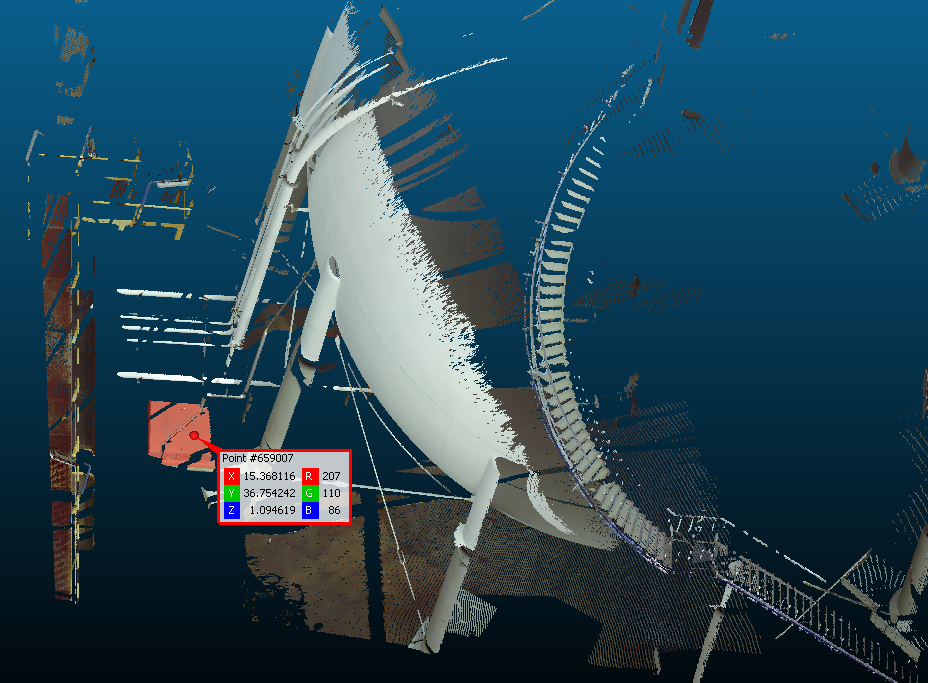
\includegraphics[width=0.8\textwidth]{./img/exemple_rgb.PNG}
    \caption{\label{} Exemple des valeurs RGB d'un point rougeâtre}
\end{figure}

Nous pouvons voir dans cet exemple, les valeurs RGB d'un point qui a été sélectionné via le point picker intégré au logiciel CloudCompare. Les valeurs en intensité sont respectivement 201-112-93. \newline

Notre première idée a donc été d'exploiter ces trois valeurs, et d'avoir un premier filtrage du nuage. Pour ce faire, nous avons réalisé un algorithme consistant à sélectionner uniquement les points qui ont des valeurs RGB proches d'un point dans le nuage. Dans nos premières itérations, nous nous basions uniquement sur la sélection d'un point, pour en définir des bornes RGB qui vont constituer notre plage de points à garder, grâce à un pourcentage d'écart. Suite à des réunions avec le client, une autre solution alternative a été de sélectionner deux points, pour directement définir nos bornes. \newline

Pour cela, nous avons développé dans un premier temps, l'interface utilisateur. Cette dernière est composée de deux points à renseigner, par leurs valeurs RGB. Afin de simplifier l'utilisation du plugin, nous avons intégré un bouton afin de sélectionner un point directement sur le nuage, et qui va ensuite renseigner les valeurs RGB du point sélectionné automatiquement. Enfin, nous avons aussi un champ afin d'écarter les limites de nos bornes RGB, pour accepter des points qui sont proches des bornes renseignées. \newline

\begin{figure}[H]
\center 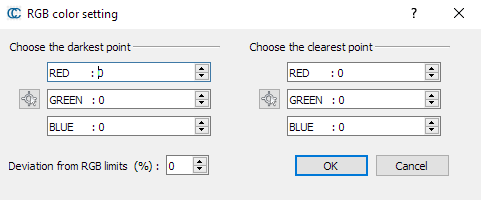
\includegraphics[width=0.8\textwidth]{./img/ui_filter_rgb.png}
  \caption{\label{} Interface filtrage RGB}
\end{figure}

Après le renseignement des bornes inférieures et supérieures en RGB, et la validation de la fenêtre, le plugin va recalculer les bornes si un pourcentage d'écart à été renseigné. Une fois ces nouvelles bornes calculées, il reste donc à parcourir l'ensemble des points du nuage, et de vérifier pour chaque point, si ses valeurs RGB sont à l'intérieur des bornes. Les points qui respectent cette condition sont gardés dans une liste de points. Cette dernière va ensuite nous servir pour créer un nouveau nuage de points.

\begin{figure}[H]
\center

\includegraphics[width=0.7\textwidth]{./img/ex_rgb_avant.PNG}
\caption{\label{} Filtrage RGB rouge : avant}
\end{figure}

\begin{figure}[H]
\center

\includegraphics[width=0.7\textwidth]{./img/ex_rgb_apres.PNG}
\caption{\label{} Filtrage RGB rouge : après}
\end{figure}

Malgré une solution qui semble fonctionner, nous pouvons quand même ressentir les limites de cette méthode. En effet, en utilisant uniquement l'espace colorimétrique RGB, nous sommes limités pour établir des vraies bornes qui permettent de séparer les couleurs plus nuancées. En effet, la qualité du filtrage dépend en grande partie des points que l'utilisateur aura sélectionné, et reste très vague en utilisant uniquement des bornes sur les valeurs RGB. C'est donc pour cela que nous avons utilisé un autre espace colorimétrique, le HSV, qui nous fournira des informations sur la teinte, la saturation et la valeur d'un point.

\subsubsection{Filtrage via l'espace colorimétrique Hue-Saturation-Value (HSV)}

Afin d'avoir plus de précisions sur la sélection de plages de couleurs, nous avons donc décidé d'utiliser l'espace colorimétrique HSV (Teinte, Saturation, Valeur en français).

\begin{figure}[H]
\center
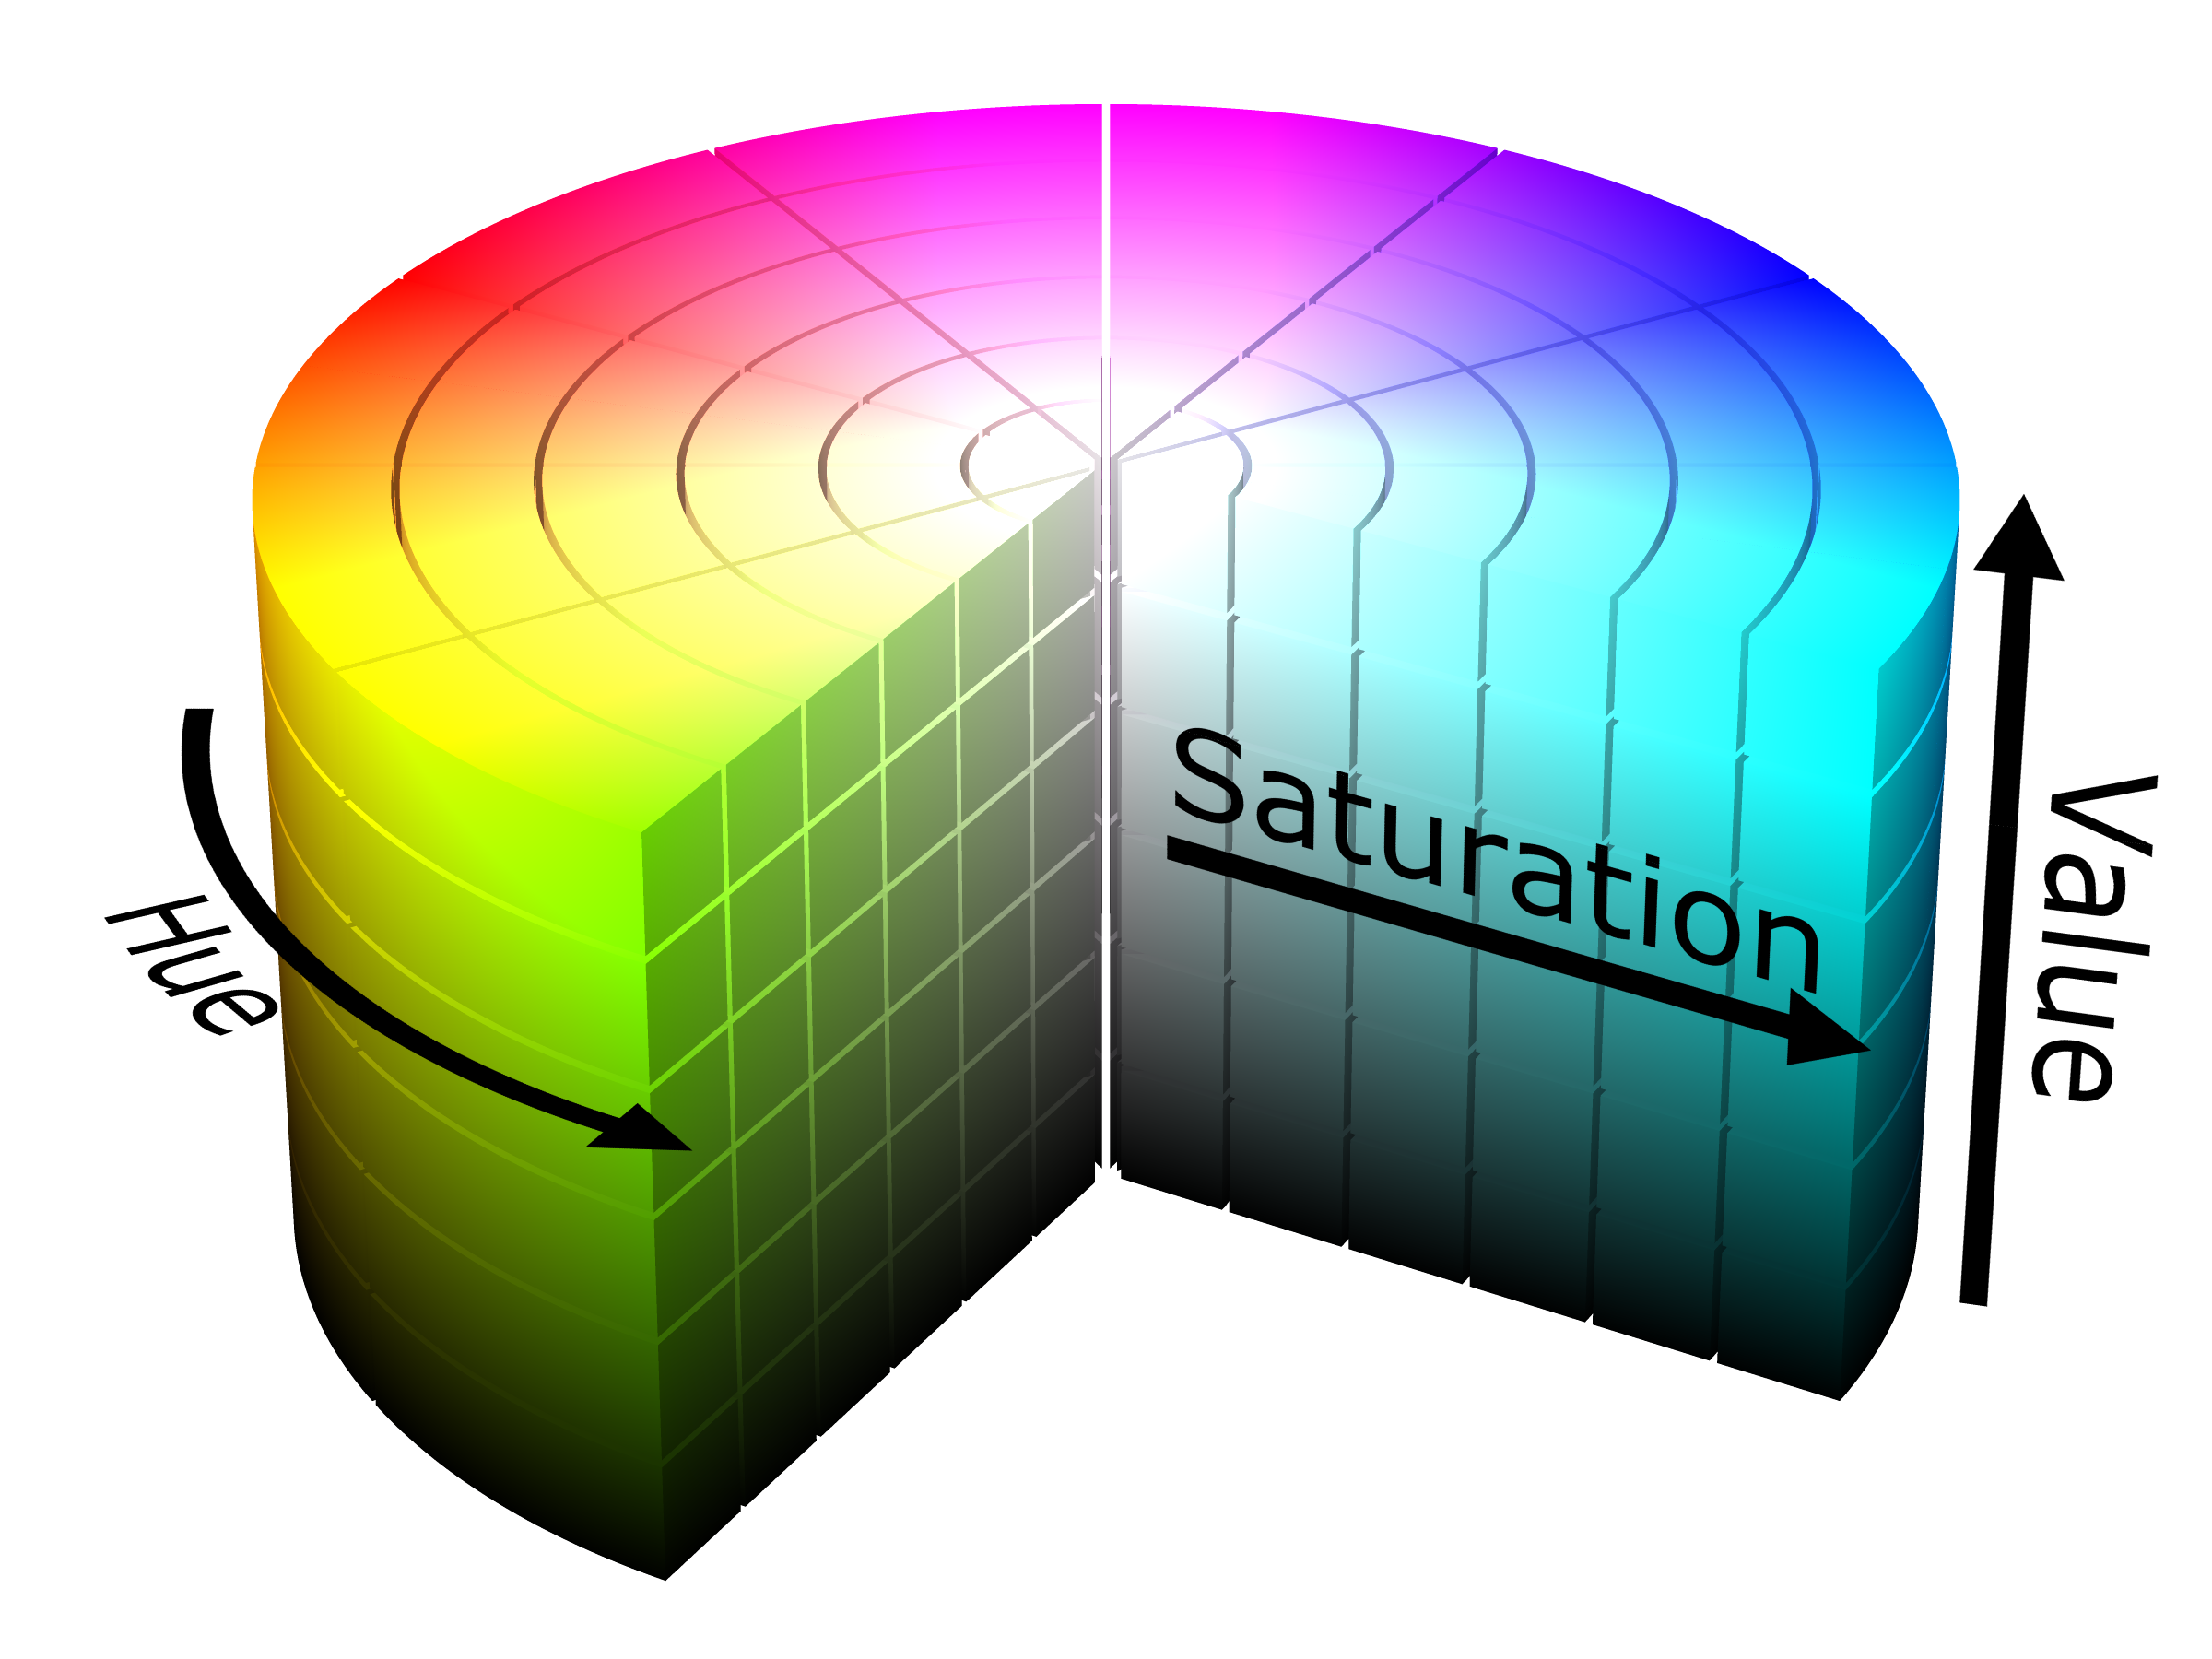
\includegraphics[width=0.7\textwidth]{./img/HSV.PNG}
\caption{\label{} Description de l'espace colorimétrique HSV}
\end{figure}

 La teinte va nous permettre de définir la couleur du point, entre 0 et 360 degrés. La saturation et la valeur, en pourcentage, nous donnent respectivement des informations sur la pureté de la couleur (0 est égal à pas de couleur, donc en nuances de gris entre le blanc et le noir, et 100 pour une couleur vive), et l'intensité lumineuse (0 pour du noir, 100 pour une couleur très claire). \newline

Pour utiliser cet espace colorimétrique, il faut convertir nos valeurs RGB d'un point, en HSV. La conversion est nommée rgb2hsv dans le fichier HSVDialog.cpp. \newline

La description de l'algorithme de conversion est disponible ici \cite{B02}. \newline

Une fois la conversion faite, nous allons pouvoir utiliser nos trois nouvelles composantes pour établir nos bornes de couleurs. Nous avons réalisé nos bornes en plusieurs étapes : \newline

Tout d'abord, nous avons commencé par analyser la composante de la saturation. Cette dernière nous permet nous dit si la couleur est vive (très "coloré"), ou pâle. Nous avons considéré qu'une saturation entre 0 et 25, sur 100, donnait une couleur pâle, donc une couleur dans les nuances de gris. Grâce à cela, nous n'avons donc pas besoin d'analyser la teinte, puisque nous savons que la couleur sera grise. \newline

Dans le cas d'une couleur grise, nous pouvons donc analyser la composante de la valeur. Ici, nous avons remarqué qu'il est donc possible de distinguer 3 couleurs principales : noir, gris et blanc. Nous avons donc défini le noir comme étant une valeur entre 0 et 25, gris pour une valeur entre 26 et 60, et blanc pour une valeur entre 61 et 100. \newline

Dans le cas où nous avons une couleur non grise, nous avons décomposé l'analyse de la valeur en deux parties seulement : une couleur noire et les autres couleurs. \newline

Une couleur noire aura une valeur entre 0 et 25. Il n'y aura donc pas besoin d'analyser la teinte. Dans le cas contraire, il faudra l'analyser pour séparer les gammes de couleurs. \newline

Concernant la dernière composante, qui est la teinte, nous nous sommes aidé du cercle chromatique, ci-dessous.

\begin{figure}[H]
\center
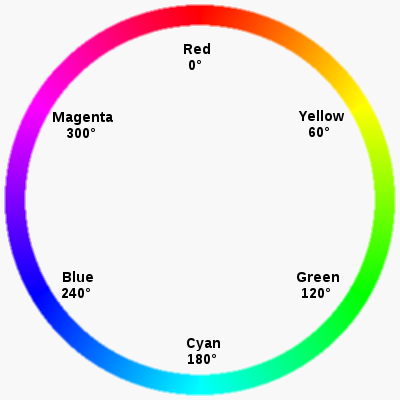
\includegraphics[width=0.7\textwidth]{./img/cercle_chromatique.PNG}
\caption{\label{} Cercle chromatique}
\end{figure}

Les plages de couleurs que nous avons fixé sont donc les suivantes :

\begin{itemize}
    \item Rouge : $0 \leq teinte \leq 30$
    \item Jaune : $30 < teinte \leq 90$
    \item Vert : $90 < teinte \leq 150$
    \item Cyan : $150 < teinte \leq 210$
    \item Bleu : $210 < teinte \leq 270$
    \item Magenta : $270 < teinte \leq 330$
    \item Rouge : $330 < teinte \leq 360$ \newline
\end{itemize}

Nous pouvons donc maintenant classifier nos points selon nos composantes HSV. Il ne nous reste donc qu'à ajouter les points qui sont de la même catégorie que le point sélectionné. Ci-dessous, un exemple de ce filtrage, identique à celui pour le RGB :

\begin{figure}[H]
\center
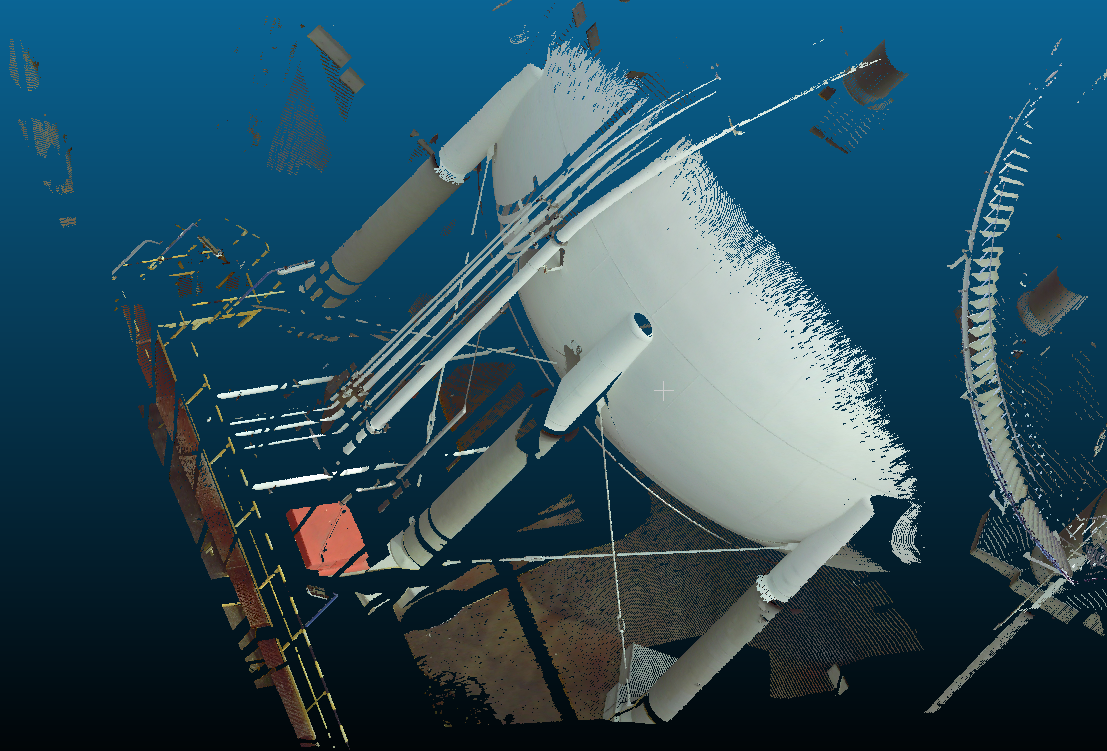
\includegraphics[width=0.7\textwidth]{./img/1_red.PNG}
\caption{\label{} Filtrage HSV rouge : avant}
\end{figure}

\begin{figure}[H]
\center
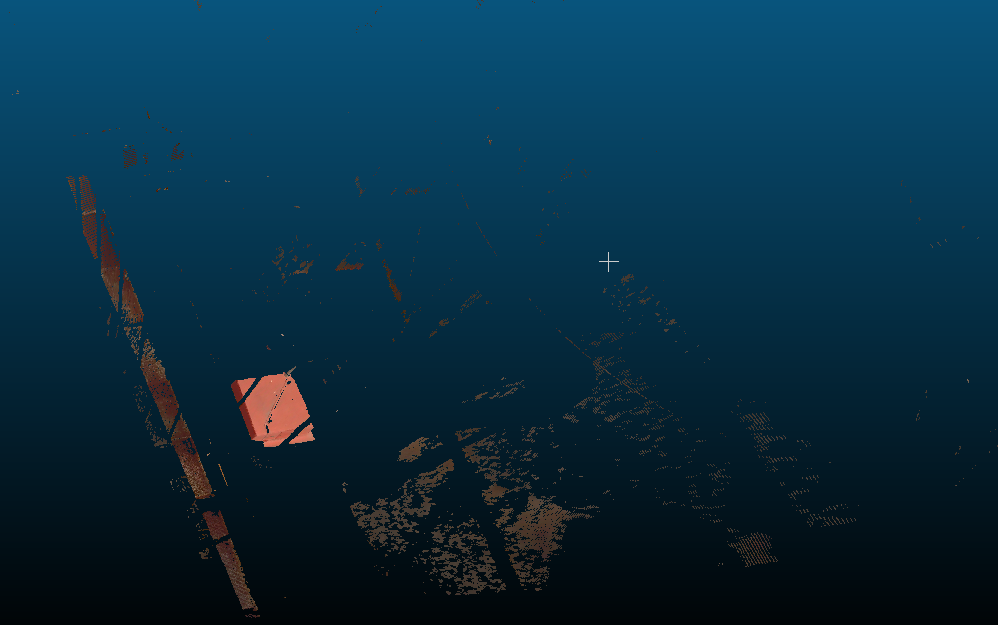
\includegraphics[width=0.7\textwidth]{./img/2_red.PNG}
\caption{\label{} Filtrage HSV rouge : après}
\end{figure}

Nous remarquons une amélioration au niveau de la sélection de tous les points rougeâtres, mais on remarque aussi qu'il y a plus de résidus. En effet, il est difficile de distinguer des points sombres de l'objet rouge que l'on veut sélectionner, des points résidus rougeâtres à cause de l'ombre. \newline

Un autre exemple sur un autre nuage de points va nous permettre de mieux voir les différences. Ci-dessous, nous allons récupérer les points blancs (RGB:255/255/255) :

\begin{figure}[H]
\center
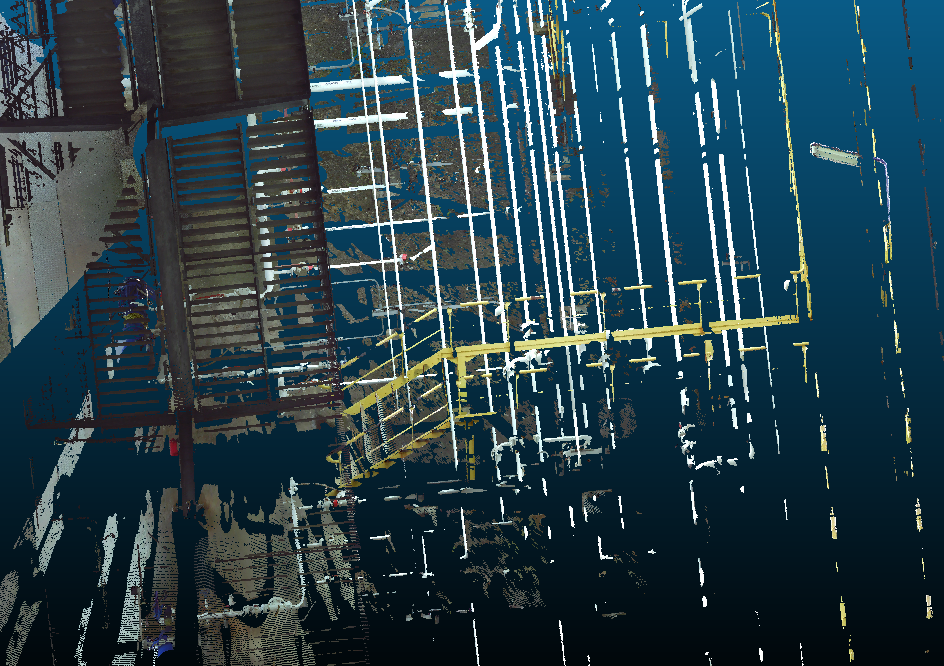
\includegraphics[width=0.7\textwidth]{./img/1_white.PNG}
\caption{\label{} Filtrage blanc : avant}
\end{figure}

\begin{figure}[H]
\center

\includegraphics[width=0.7\textwidth]{./img/3_white.PNG}
\caption{\label{} Filtrage RGB blanc : après}
\end{figure}

\begin{figure}[H]
\center

\includegraphics[width=0.7\textwidth]{./img/2_white.PNG}
\caption{\label{} Filtrage HSV blanc : après}
\end{figure}

Nous remarquons donc une nette amélioration au niveau de la sélection des tuyaux blancs, surtout pour les tuyaux qui ont une couleur blanche mais avec un peu d'ombre. Même si on obtient des résidus, nous pouvons maintenant récupérer avec plus de précision les points que nous voulons. \newline

Les limites de cette méthode sont que les plages de couleurs sont fixes dans le code. Il serait possible d'afficher un mode "avancé" pour l'utilisateur, afin qu'il puisse définir lui-même ses bornes. Après discussion avec les demandes du client, cette option étant facultative et avec un manque de temps sur le projet, nous n'avons pas développé cette partie.

\newpage
\section{Conclusion et perspectives}

Pour conclure sur ces itérations, de façon générale, nous avons pu suivre en grande partie ce que nous avions prévu sur le cahier des charges. La majorité des Users Stories ont été développés et validés par le client. Arrivant à la fin du projet, nous avons pu améliorer ce que nous avions développé dans la version alpha, et terminer les tâches en cours.\newline

La première itération nous a permis de nous conforter sur le développement futur de notre solution, et les deux itérations suivantes nous ont permis de poser les bases, et de commencer à donner une solution viable. Pendant la quatrième itération, nous avons consolidé ce que nous avions développé, puis nous avions préparé une première version du projet pour le client pendant la cinquième, qui a pu nous faire des retours côté utilisateur. Enfin la dernière itération a été dédié à des correctifs, et la fin des tâches en suspend. \newline

Durant la première itération, nous avons de nombreuses questions sur le développement de notre projet. Nous avions notamment le choix du langage, la façon de développer nos algorithmes, l'implémentation, etc. C'était une itération où nous n'avions pas produit de contenu direct pour le client, mais nous avions pu partager nos recherches et de nos choix. Nous avions donc décidé de développer notre solution en C++, avec un plugin CloudCompare. \newline

La recherche d'algorithmes de segmentation nous a permis de gagner du temps sur l'implémentation, afin d'éviter de changer entre phases de recherche, et phases d'implémentation, sur une même itération. Ainsi, cela nous permettait de mieux se concentrer sur la phase d'implémentation. \newline

Toutefois, nous avons quand même pris du retard notamment sur la deuxième et troisième itération. Lors de la deuxième itération, nous pensions que nous pourrions avoir une meilleure base de notre plugin sur CloudCompare, afin de pousser l'implémentation des algorithmes de segmentation. Malheureusement, nous avions rencontré des difficultés par rapport à la création d'un nouveau plugin. Ce temps perdu a donc impacté le développement de la troisième itération, qui consistait à l'amélioration de ce que nous avions développé, et l'implémentation de nouveaux algorithmes. \newline

Lors de la troisième itération, nous avions préféré se concentrer sur l'amélioration de notre code par rapport à l'implémentation de nouvelles fonctionnalités, car il nous semblait important d'avoir une structure stable et facile à maintenir, pour la suite du projet. Grâce à cela, nous avons maintenant un plugin indépendant aux autres, qui est totalement fonctionnel, et qui peut facilement ajouter des nouveaux algorithmes de segmentation. \newline

De plus, nous avons quand même pris en compte le feedback du client, afin d'améliorer notre solution, par rapport à son utilisation. Ici, c'était principalement lié à l'interface des algorithmes de segmentation. Nous avons apporté des modifications notamment sur le point picking, très important pour faciliter l'utilisation de notre plugin (au lieu de rentrer manuellement les valeurs à filtrer), ou encore des changements sur la plage de couleur à prendre, etc. \newline

Nous avions rencontré beaucoup de difficulté pour fournir la première version du projet à notre client, notamment à cause des problèmes de compatibilité des versions, par rapport au logiciel CloudCompare, Qt, ou encore la version du SDK de windows. En effet, nous compilions avec une version plus récente de Visual Studio (2019), qui utilisait donc une version SDK windows plus récente que les machines de notre client. Le seul moyen de savoir d'où venait le problème était de notre côté, tester différentes solutions, puis de les fournir au client afin qu'il puisse réaliser les tests. En prenant en compte les délais de communication, nous avions perdu du temps. \newline

Une fois ce problème résolu, il a nous été assez facile d'avancer sur le projet, tout en prenant en compte le feedback du client qui pouvait utiliser le plugin pour des cas réels. \newline

Même si l'ensemble des tâches ont été validées, le projet peut encore être améliorable. En effet, nous avons, par exemple, la version avancé du filtrage HSV, pour qu'un utilisateur plus expérimenté puisse affiner sa sélection de points. \newline

Ce projet sera, à terme, un plugin qui fera partie des autres plugins de CloudCompare. Un contact a déjà eu lieu avec M. Daniel Girardeau-Montaut, afin de discuter dans un premier temps sur les règles à respecter.

\newpage
\section{Annexes}

Les annexes contiendront tout ce qui ne concerne pas directement la description du système. Nous allons décrire le déroulement du projet transversal, et réalisant une rétrospection sur nos itérations. De plus, nous fournirons le rapport de recette.

\subsection{Déroulement du projet}

Il est important de faire un retour sur le déroulement du projet, afin de savoir ce que nous avons bien réalisé, les difficultés que nous avons rencontrés, nos méthodes de travail, etc. En effet, cela nous permettra d'améliorer nos démarches pour mener à bien ce projet. 

\subsubsection{Vision globale du projet}

D'un point de vu global sur le projet, nous avons rencontré certaines difficultés, mais aussi appris beaucoup par rapport au fonctionnement d'un projet agile. \newline

Tout d'abord, il a été difficile d'estimer notre charge de travail. Comme c'était notre premier vrai projet en lien avec une autre entreprise, et d'une aussi grande envergure (durée d'un an), il nous fallait en quelque sorte expérimenter notre capacité de travail et d'évaluer les tâches à réaliser. \newline

Certaines tâches furent plus difficiles à réaliser, par rapport à nos prévisions. Par exemple, nous pouvons citer l'implémentation d'un nouvel algorithme de segmentation, plus complexe, ou encore l'implémentation d'un point picking. Le temps prévu à consacrer sur ces types de tâches n'était pas assez important, car nous avions mal pris en compte les autres tâches en parallèle, hors projet. Ces autres tâches était notamment d'autres projets sur de courtes durées, devoir surveillées, oraux, etc. \newline

Nous nous sommes aussi rendu compte que les itérations se déroulent très vite. Pour chaque itération, nous étions surpris par le fait qu'un mois s'était passé. Grâce aux réunions planifiées avec le client et le tuteur académique, nous pouvions quand même garder une bonne dynamique pour respecter les deadlines. \newline

De plus, la mise en situation d'un projet agile nous a fait prendre conscience de l'importance de garder le client au courant, afin d'avancer correctement par rapport aux besoin de celui-ci. Mais pour cela, il faut rédiger de nombreux rapports. Ce sont des tâches qu'il ne faut pas sous-estimer, puisque cela demande beaucoup de temps. Même si les réunions aident à transmettre l'avancement du projet et des tâches réalisées, il faut aussi écrire formellement dans un rapport l'avancement pour garder une trace de ce qui a été fait. \newline

La rédaction des rapports d'itération, et des rapports hebdomadaires, sont difficiles à maintenir. En effet, nous avions eu parfois des difficultés à suivre le rythme des rapports hebdomadaires. Malgré tout, cela reste nécessaire notamment pour avoir un historique de l'avancement des tâches, et des heures passées sur chacune d'entre elles.

\subsubsection{Comparaison de la planification des itérations}

Nous avons aussi réalisé un comparatif de la planification de nos itérations, avec ce qu'il s'est réellement passé. Nous avons donc comparé le temps passé sur chacune des tâches, entre nos prévisions et la réalité. Cela nous permettra d'analyser les problèmes rencontrés, et d'améliorer par la suite notre capacité à évaluer notre charge de travail. \newline

Afin de faire ressortir les tâches qui nous ont pris plus ou moins de temps que prévues, nous avons utilisé un code couleur, disponible ci-dessous :

\begin{figure}[H]
\makebox[\textwidth][c]{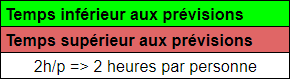
\includegraphics[width=0.4\textwidth]{./img/legende.PNG}}
    \caption{\label{} Légende tableaux Gantt}
\end{figure}


\begin{figure}[H]
\makebox[\textwidth][c]{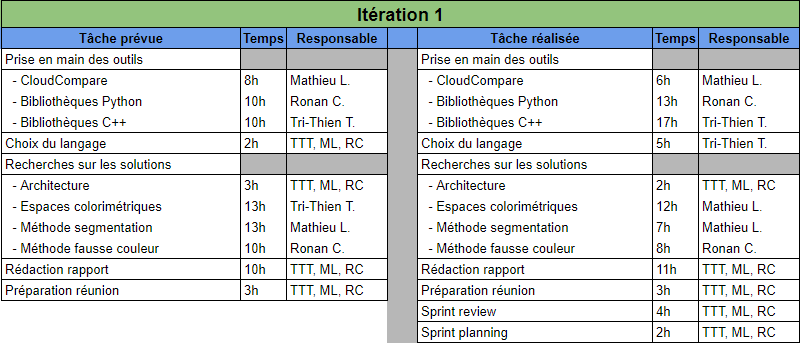
\includegraphics[width=1.2\textwidth]{./img/gantt_1.PNG}}
    \caption{\label{} Comparaison Gantt de l'itération 1}
\end{figure}

Ce premier tableau nous montre les tâches que nous avions prévues pour notre première itération, représentées du côté gauche, avec la tâche prévue, le temps estimé et le responsable de la tâche. De l'autre côté, nous pouvons observer les mêmes tâches, avec le temps réellement passé pour les réaliser. \newline

Nous pouvons voir que le temps réellement passé ne correspond pas du tout à ce que nous avions prévu. En effet, comme c'était notre première itération, il nous a été difficile d'estimer notre capacité de travail, et du temps à passer sur chacune de nos tâches. \newline

Nous pouvons aussi observer que sur la tâche des recherches sur les espaces colorimétriques, le responsable a été changé, de même que pour le choix du langage. Pendant notre avancée sur l'itération, nous nous sommes rendu compte que certaines tâches étaient plus rapide à réaliser que d'autres, par exemple sur la prise en main de CloudCompare, ou encore sur les méthodes de segmentation. Ce gain de temps nous a permis d'attribuer la responsabilité de travailler sur les espaces colorimétriques à Mathieu L, et libérer du temps à Tri-Thien T. pour se concentrer sur d'autres tâches. Ce dernier a eu beaucoup de temps supplémentaires à attribuer sur ses tâches, notamment car c'est un travail de recherches, donc cela nécessite beaucoup de documentations, donc beaucoup de temps. De plus, il fallait ensuite produire un rapport facile à comprendre pour les autres membres du groupe, et pour le client. \newline

De plus, nous avions des tâches qui n'étaient pas prévues dans nos prévisions, mais qui étaient présentes en réalité. Nous pouvons citer la préparation du Sprint review, ou encore le sprint planning. C'est pour cela que ces tâches n'apparaissent pas dans les tâches prévues, mais uniquement dans les tâches réalisées.

\begin{figure}[!hbtp]
\makebox[\textwidth][c]{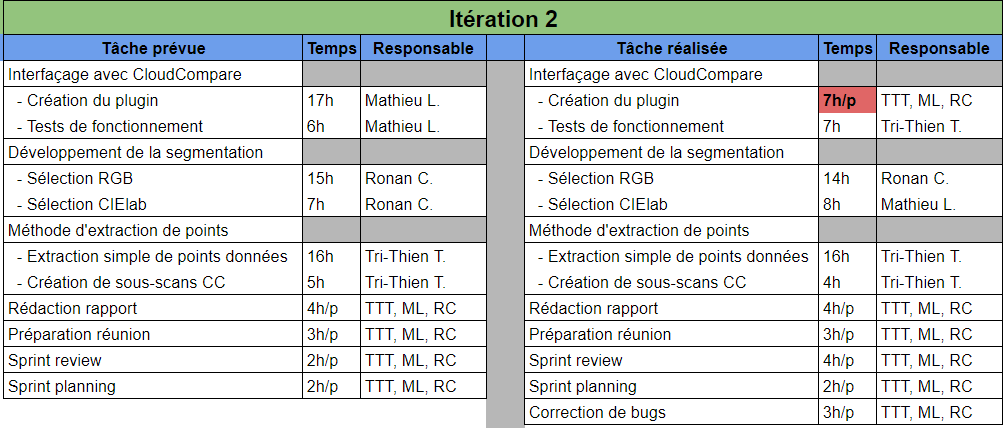
\includegraphics[width=1.2\textwidth]{./img/gantt_2.PNG}}
    \caption{\label{} Comparaison Gantt de l'itération 2}
\end{figure}

Pour la deuxième itération, les prévisions du nombre d'heures par tâches ont plutôt bien été respectées, sauf pour la partie sur l'interfaçage avec CloudCompare. En effet, cette partie était concentrée sur l'implémentation d'un nouveau plugin sur le logiciel CloudCompare. Nous avions un tutoriel à notre disposition pour l'installation, mais nous avions rencontré beaucoup de problèmes. Nous pouvons par exemple citer les différents logiciels à installer au préalable (QT, PCL...), qui sont très volumineux et prennent beaucoup de temps à installer. Ensuite, il faut savoir comment les utiliser, ce qui demande une phase de formation sur les outils. \newline

Une fois ceci fait, il fallait ensuite créer notre propre interface et nos propres algorithmes de traitement sur le nuage de points. Une fois encore, il fallait que l'on se forme sur comment un plugin CloudCompare fonctionne, sa structure et comment ajouter notre propre code.

\begin{figure}[!hbtp]
\makebox[\textwidth][c]{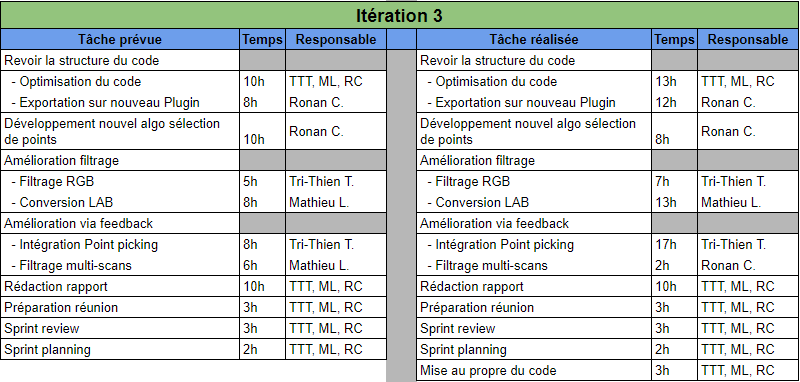
\includegraphics[width=1.2\textwidth]{./img/gantt_3.PNG}}
    \caption{\label{} Comparaison Gantt de l'itération 3}
\end{figure}

Cette troisième itération était dédiée à l'amélioration de notre solution, et surtout de revoir la structure de notre code pour avoir une meilleure organisation. De même que pour la première itération, nous avons eu ici du mal à bien estimer la durée de nos tâches. Les principales différences entre le prévisionnel et le réalisé est le fait que nous ne connaissons pas encore assez le code du projet CloudCompare, donc ne savons pas vraiment ce qui est possible de faire avec les outils du projet ou non. \newline

De plus, nous avons rencontré des difficultés pour obtenir des résultats satisfaisants, notamment pour la conversion LAB, et des difficultés à comprendre le fonctionnement d'un plugin sur le logiciel CloudCompare, notamment le principe des signaux et des slots en C++ (pour l'implémentation d'un point picking). \newline

Il faut aussi noter que pour le développement d'un nouvel algorithme de sélection de points dans le nuage, la durée indiquée ici ne veut pas dire que la tâche est terminée. En effet, la tâche est plus compliquée que prévu, et malgré le temps donné à cette tâche, il faut encore y attribuer du temps pour la finaliser.

\subsection{Rapport de recette}

Cette section sera présente pour le rapport final de la description du système (version beta).
\begin{thebibliography}{3}
  \bibitem{B01} Qingming Zhan, Yubin Liang, Yinghui Xiao, \textit{Color-based segmentation of point clouds}, 2009
  \bibitem{B02} Conversion RGB - HSV : \url{https://mattlockyer.github.io/iat455/documents/rgb-hsv.pdf}
\end{thebibliography}
\end{document}
